\section{Software}
\label{sec:chapterexample}

\subsection{Programmiersprachen}
Das System besteht aus mehrere Programme und Dienste. Für die Entwicklung werden folgende Programmiersprachen eingesetzt:
\begin{itemize}
	\item Java
	\item Javascript
	\item PHP
\end{itemize}
Im Verbindung mit PHP kommt natürlich die Markup-Languages HTML5/CSS, welche für die graphische Darstellung der Webapplikationen notwendig ist.

\subsubsection{Java}
\label{kap:java}
Alle Dienste die Serverseitig und ohne Interaktion mit dem Enduser ausgeführt werden, werden in Java programmiert. Als stark typisierte und Objektorientierte Programmiersprache eignet sich Java für dieses Projekt. Für Java sind auch unzählige Libraries verfügbar, insbesondere für die Hardware Steuerung der Raspberry Pi. Eine zweite Variante wäre Python gewesen, die auch das Raspberry sehr gut unterstüzt. Python ist aber zu wenig typisiert und für eher kleinere Softwarestücke gedacht.

\subsubsection{PHP/Javascript}
Die Client Applikation sowohl auch die Applikation bei der Aussensprechstelle werden Web-Applikationen sein. Dies ermöglicht eine schnelle und zeitgemässe Softwareentwicklung. Für dieses Projekt ist die System-Eingriffstiefe von Webapplikationen jedenfalls ausreichend. Es muss lediglich Zugriff auf Mikrofon, Lautsprecher und Kamera garantiert werden. Ein weiteres Punkt zugunsten einer Webapplikation ist die Cross-Plattform Kompatibilität.
\\
Aus diesem Grund haben wir uns für PHP (Objektorientiert) im Kombination mit Javascript/HTML/CSS entschieden. Eine zweite Variante wäre Java EE gewesen. Java EE eignet sich aber vor allem für grosse Softwarelösungen und bietet als gesamten Framework vieles mehr als was dieses Projekt benötigt.
\\
\subsubsection{PHP Framework: Laravel}
Für die Entwicklung der Webapplikationen wird Laravel als PHP Framework eingesetzt. Laravel ist ein Open-Source PHP Web-Application-Framework, die sich für kleine bis zu mittelgrosse Projekte eignet. Laravel beruht auf dem Modell-View-Controller-Muster und ermöglicht eine Objektorientierte Programmierung in PHP.

\subsection{System Übersicht}
Das System besteht aus mehrere Hardware- und Softwarekomponenten die zusammenarbeiten müssen (\seeref{fig:echosystem}). Die  Vertraulichkeit der Kommunikation zwischen den Knoten ist von TLS immer gewährleistet. Die einzelne Komponenten, sowie das Thema Sicherheit, werden in den nächsten Kapiteln genauer beschrieben.

\begin{figure}[htb!]
	\begin{center}
		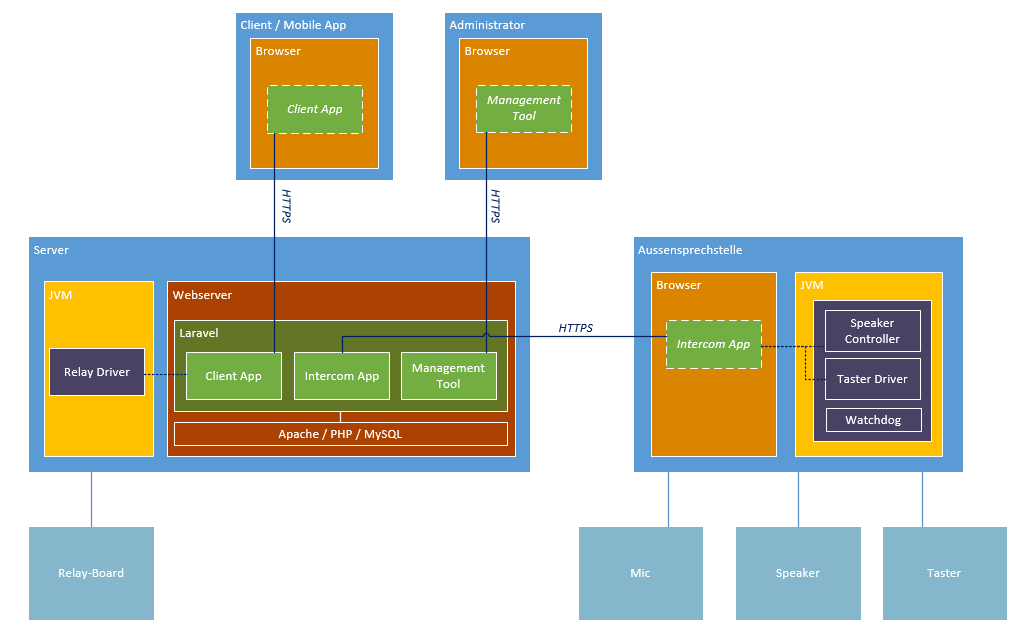
\includegraphics[width=1\textwidth]{ecosystem}
		\caption[Software / Hardware Ecosystem]{Software / Hardware Ecosystem}
		\label{fig:echosystem}
	\end{center}
\end{figure}

Die Software wird in zwei Gruppen unterteilt. Einerseits gibt es alle Dienste/Daemons \textit{(Violett)} die Lokal ausgeführt werden und quasi das Backend des Systems darstellen.
\\
Die zweite Gruppe beinhaltet die Webapplikationen \textit{(Grün)}, die eine GUI besitzen und für die Interaktion mit dem System gedacht sind. Darunter zählen die Client-App für den Bewohner, die Applikation bei der Aussensprechstelle wo die Bewohner angezeigt werden und das Management Tool.
\\
Die Audio/Video-Kommunikation zwischen die Aussensprechstellen und die Client-Apps wird mithilfe von WebRTC realisiert. Diese hat eine gewisse Komplexität und wird in ein eigenes Kapitel (\seeref{kap:webrtc}) behandelt.

\subsection{Raspbian}
\label{kap:raspbian}
Auf alle Raspberry Pi wurde den Betriebssystem Raspbian Jessie installiert. Diese wird von Raspberry Pi Foundation mitgeliefert und gilt als besonders hochoptimerte OS für die mit niedriger Leistung und geringem Stromverbrauch ARM Prozessoren.
Der Raspbian Jessie Betriebssystem basiert auf Debian welch unter der DFSG (Debian Free Software Guidelines) Lizent steht. Diese erlaubt der unbeschränkte Weitergabe des Software sowie abgeleitete und modifizierte  Werke weiterzugeben. 
Raspbian enthält Java SE Platform Prudukte welches und dem BCL(Oracle Binary Code License) lizensiert sind. Dieses Lizenz gewährleistet die obengenannten Freiheite ebenfalls.

\subsection{Dienste}
\label{kap:dienste}

\subsubsection{Taster Controller}
Die Aussensprechstelle wird durch 3 Schalter bedient. Die drei Schaltern werden an die GPIO-Pins des Raspberry PI angeschlossen. Die Aufgabe der Taster-Controller besteht darin, die GPIO-Input Signale, als verwendbare Tastatur-Eingaben umzuwandeln. Somit kann die GUI an der Aussensprechstelle gesteuert werden.
\\
Die ursprüngliche Idee war das Taster-Controller, so wie alle andere Dienste, als Daemon auszuführen. Das hätte den Vorteil, dass der Daemon mittels die übliche run, stop und restart Befehle gesteuert werden könnte. Eine der eingesetzten Java-Library benötigt aber den zugriff auf dem Graphisches Umgebung. Das Problem besteht darin, dass ein Daemon Benutzer-Unabhängig ist, während der X-Server beim Login einem Benutzer ausgeführt wird. Das ausführen der Deamon erst ab Init 5, da wo auch der X-Server ausgeführt wird, konnte aus diesem Grund das Problem auch nicht lösen.
Die verwendete Library hat also keine Möglichkeit, als Deamon eine Verbindung mit dem X-Server aufzubauen.
\\\\
Die Desktop-Umgebung LXDE welche von Raspbian verwendet wird, bietet aber ein Autostart welches das Taster-Controller nach dem Initialisierung des X-Server, unter dem gleichen Benutzer ausführt.

\subsubsection{Speaker Controller}
Das Speaker Controller ist ein kleinen Dienst, welche den Lautsprecher ein- und ausschalten kann. Trotz einem Massentrennfilter sind immer noch leise Störsignale auf der Audio-Ausgang vorhanden.
Die Aufgabe des Speaker-Controllers besteht darin, die Stromspeisung des Speakers zu trennen, wenn es nicht verwendet wird. Somit ist das System Energieeffizienter und unnötige Geräusche können vermieden werden.
\\
\\
Der Dienst besteht lediglich aus ein Socket-Server, der auf ein Signal wartet und durch die GPIO der Raspberry, ein kleines Relay steuert.
Das Signal kommt von der Aussensprechstelle-Applikation \textit{(localhost)}. So kann den Lautsprecher bei Bedarf ein- und ausgeschaltet werden.

\subsubsection{Relay Controller}
...
\subsubsection{Signaling Server}
Der Signaling-Server ist ein bestandteil von WebRTC und wird in ein eigenes Kapitel ausführlich beschrieben (\seeref{kap:signaling}).

\subsection{Logging}
\label{kap:logs}
Für die Identifikation und Rückverfolgung von Fehlern sowie für den Monitoring sind Logs File von grosse Bedeutung. Diese werden bei allen Services und Dienste konsequent druchgeführt. Das Logrotate wird nicht eingesetzt, statdessen kümmert sich das Java runtime environment um die Grösse des generiertes Log File. Aus dem Grund dass es sich noch um ein Protoyp handelt wurde das Logging Stufe auf 7 eingestellt. In diese Stufe werden alle Emergency Nachrichten bis auf die Debug Nachrichten im Log Dateien gespeichert.
Gemäss der FHS (Filesystem Hierarchy Standard) werden die Logs unter /var/log/Aussensprechstelle gesichert. 

\subsection{Watchdog}
\label{kap:watchdog}
Die ganze Hardware, die an die Türe installiert wird, ist bei eine Endkunde schwer zugänglich. Sollte nun ein Problem mit dem System auftreten, müsste man Vorort die Anlage zurücksetzen. Die Lösung heisst hier Hardware-Watchdog, die auf dem Raspberry komplett unabhängig vom eigentlichen System läuft. Der Vorteil von ein Hardware-Watchdog ist das wenn der System bzw. der Prozessor steht, führt diese unabhängige Hardware ihre Aufgabe weiterhin aus.
Der Watchdog wird als standalone Gerät im Unix erkennt. Wird diese Gerät einmal beschrieben, dann muss diese im eine Zeitintervall von 15 Sekunden erneut beschrieben werden. Ist diese Bedingung nicht erfüllt, denn wird ein Hardware-Reset von Watchdog durchgeführt und das System wird neugestartet.
Das Beschrieben von der Watchdog-Gerät wird von eine Watchdog-Daemon übernommen. 
Durch der Konfigurationsdatei des Daemon können verschiedene Parameter des System wie Temperatur, Auslastung der Prozessor usw. überwacht werden. Besonders relevant für die Türsprechanlage ist das PID-Monitoring. Diese ermöglicht das ständig überprüfen von spezifische Prozesse und Diensten die das System benötigt, um sein Zweck als Aussensprechstelle zu erfüllen. Sobald eine diese Prozesse steht wird das System innerhalb von 15 Sekunden nuegestartet. 
Ein solches Mechanismus steigert die Verfügbarkeit des Dienst, die für eine Türsprechanlage von grosse Bedeutung ist.
\subsection{Webapplikationen}
\label{kap:webapp}


\subsubsection{Client Webapplikation}
Der Bewohner muss über eine Applikation verfügen, die auf dem Tablet oder Handy ausführbar sein muss. Mithilfe dieser App muss der Enduser folgendes können: Sich mit alle Aussensprechstellen verbinden können, ein Video Signal von der Kamera aller Eingänge erhalten, alle Türe öffnen und mit der Person bei der Türe über die Anlage kommunizieren können.
\\
\begin{figure}[htb!]
	\begin{center}
		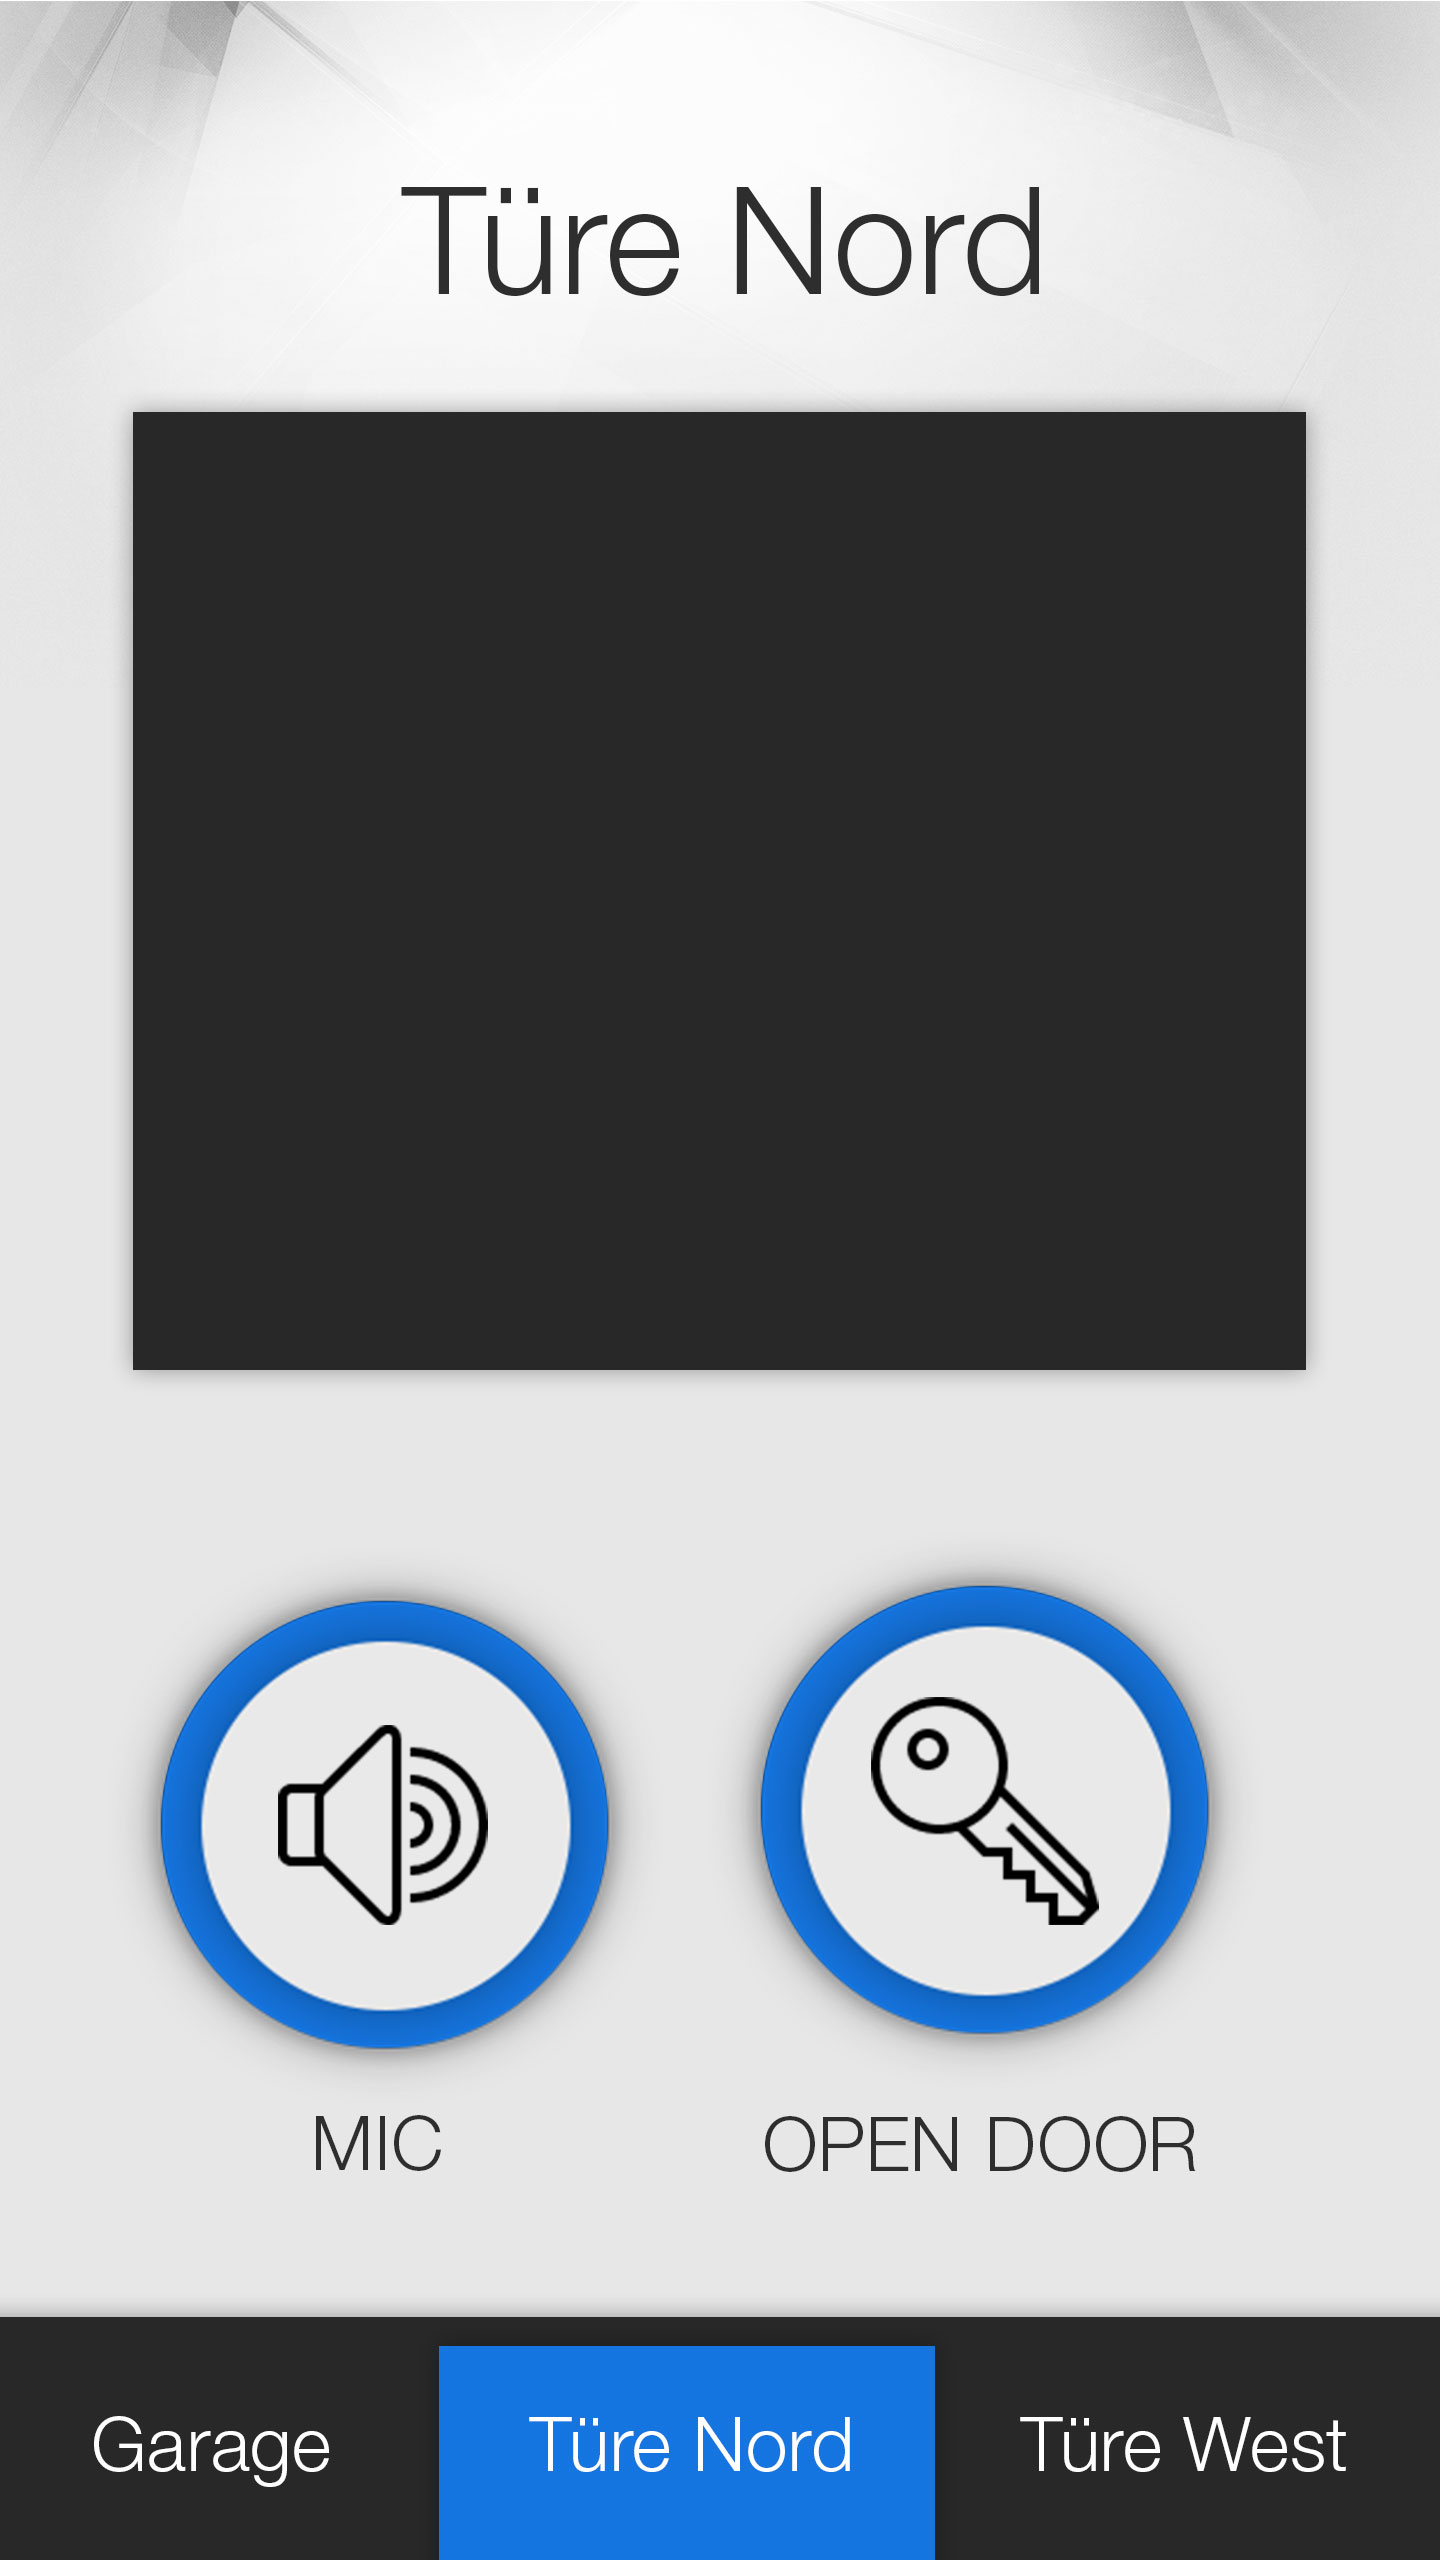
\includegraphics[width=0.35\textwidth]{clientDemo}
		\caption[Design der Client-Webapp]{Design der Client-Webapp}
		\label{fig:clientDemo}
	\end{center}
\end{figure}
\\
Die \cref{fig:clientDemo} zeigt das Design für die Webapplikation. Hier gezeigt ist die Smartphone Version. Dank ein Responsive-Design wird die selbe Applikation auch auf andere Geräte wie z.B. Tablets oder Computers passend angezeigt.
\\ 
Bei der Design-Entwurf standen Übersichtlichkeit und Benutzerfreundlichkeit im Vordergrund. Aus diesem Grund werden die Tasten für die Audio-Kommunikation und für die Öffnung der Türe gross Angezeigt. Das Videostream von der ausgewählte Türe wird sofort angezeigt und benötigt keine weitere Interaktion. 

\subsubsection{Aussensprechstelle Webapplikation}
..

\subsection{Management Tool}
\label{kap:managementtool}
..

\subsection{WebRTC}
\label{kap:webrtc}
WebRTC ist ein offener Standard, der eine Sammlung von Kommunikationsprotokollen und API beinhaltet. Die Standardisierung wird mehrheitlich betrieben und unterstützt von Google, Mozilla Foundation und Opera Software. WebRTC basiert auf HTML5 und Javascript und die Audio/Video Übertragung erfolgt über eine direkte Verbindung zwischen den Sprechpartner (Peer-to-Peer).
\\
\\
WebRTC wird hauptsächlich für die Entwicklung von Videokonferenz Programme verwendet. Die Natur dieses Projekt ist allerdings nicht dieselbe wie die herkömmliche Real-Time-Communication Applikationen. Glücklicherweise wurde WebRTC so entwickelt, um möglichst viel Flexibilität zu garantieren. Aus diesem Grund beinhaltet der WebRTC-Standard keine Definition für den Signaling-Process, welcher zusammen mit dem ICE (Interactive Connectivity Establishment) für den Verbindungsaufbau zwischen den Sprechpartnern zuständig ist. 

\begin{quote}
	\textit{
		"The thinking behind WebRTC call setup has been to fully specify and control the media plane, but to leave the signaling plane up to the application as much as possible. The rationale is that different applications may prefer to use different protocols, such as the existing SIP or Jingle call signaling protocols, or something custom to the particular application, perhaps for a novel use case. [...]"
	} 
	\\
	\cite[Sam Dutton, HTML5Rocks.com]{001} 
\end{quote}

\subsubsection{Signaling Process}
\label{kap:signaling}

Ähnlich wie bei VoIP-Telefonie \textit{(SIP)}, brauchen die Sprechpartner ein gemeinsam bekanntes Knoten, um die Verbindung zu initialisieren (\seeref{fig:signaling}). In den meisten Fällen ist einem Partner, die logische Adressierung der andere Partner nicht bekannt. Es besteht also keine Möglichkeit um eine P2P Verbindung auf einmal zu starten.
\begin{figure}[htb!]
	\begin{center}
		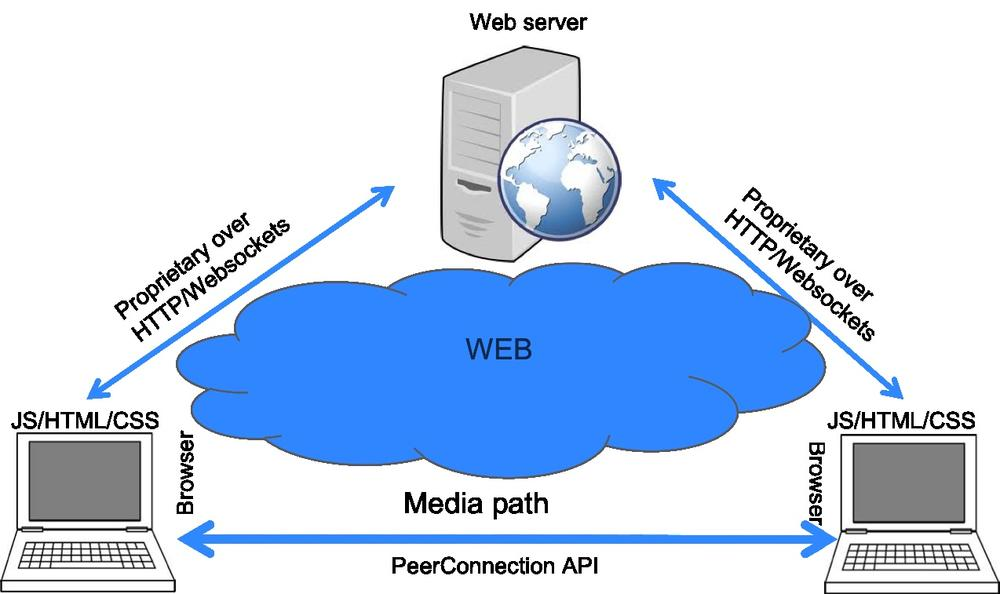
\includegraphics[width=0.75\textwidth]{signalingprocess}
		\caption[Der Signaling Prozess]{Der Signaling Prozess}
		\label{fig:signaling}
	\end{center}
\end{figure}
\\
Im unseren Fall wäre es theoretisch möglich, da die Position der Aussensprechstellen bzw. der Server immer dieselbe sind. Allerdings wurde WebRTC nicht so konzipiert. Die Standard WebRTC API beinhaltet kein Konstrukt um eine Verbindung anhand von Bekannter IP-Adresse aufbauen zu können.
\\
Im Internet sind es mehrere Signaling-Server Libraries verfügbar. Allerdings sind diese für andere Anwendungen gedacht. Im unseren System, wird beispielsweise nie eine Anruf von der Aussensprechstelle zu den Client-App gestartet, sondern lediglich umgekehrt.
\\
Für die Zwecke unser Projekt wurde ein eigenes Signaling-Server entwickelt. Dieser wird auf den Server ausgeführt und somit bleibt der Datenverkehr zwischen dem Client-App und der Aussensprechstelle, während jeder Schritt der Verbindungsaufbau und Kommunikation, innerhalb des lokales Netzwerkes. Das natürlich nur, solange der Bewohner sich zu Hause befindet.

\subsubsection{STUN Servers \& Remote Verbindung}
\label{test}
Eine Anforderung des Systems ist die Möglichkeit, auch ausserhalb des Heimnetzes mit den Aussensprechstellen sich verbinden zu können. Hier stellt das NAT-Protokoll (Network Adress Translation) ein Problem dar.
\\
Nach dem Signaling-Prozess wird das ICE-Prozess gestartet. Hier tauschen sich die zwei Partner Informationen über die eigene Adressierung und den \textit{best path} aus. Falls sich ein Sprechpartner hinter ein NAT-Knote befindet, wird für den anderen unmöglich sein eine Verbindung aufzubauen. Hier kommen die STUN-Servers im Spiel. Ähnlich wie bei dem Signalisierungsprozess stehen STUN-Servers als Hilfe für den Verbindungsaufbau da (\seeref{fig:stun}).
\begin{figure}[htb!]
	\begin{center}
		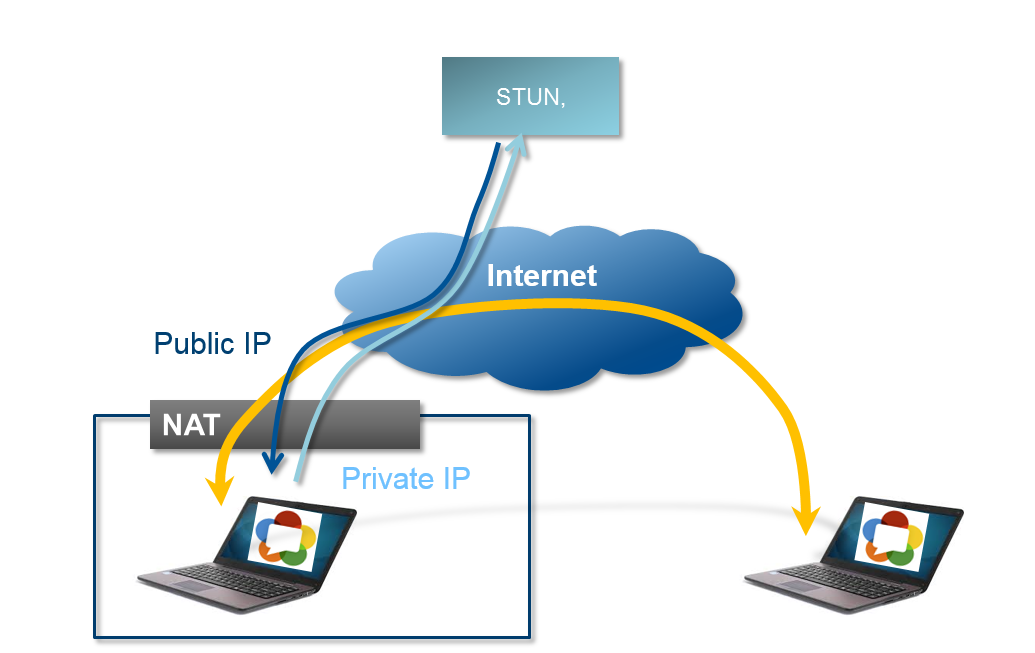
\includegraphics[width=0.75\textwidth]{stun}
		\caption[STUN Server]{STUN Server}
		\label{fig:stun}
	\end{center}
\end{figure}
 STUN-Servers informieren die Clients über jegliche NAT Konfigurationen die sich dazwischen befinden würden. Die beide Sprechpartner erhalten somit Informationen über welche Ports und Öffentliche Adressen die Verbindung initialisiert werden kann. Für die Entwicklung dieses Projektes werden die Google STUN Servers verwendet, welche kostenfrei zur Verfügung stehen.
\\
Falls sich beide Sprechpartner im gleichen lokales Netzwerk befinden, werden keine STUN-Servers benötigt und den gesamten Datenverkehr bleibt innerhalb des Heimnetzwerkes.

\newpage